\appendix
\section{Data details}
\label{app:data}
\textbf{Hands per stake} (6-max PartyPoker tables kept): 1{,}338{,}547 at \$0.10/\$0.25, 659{,}208 at \$2/\$4, 278{,}612 at \$3/\$6 and 365{,}025 at \$5/\$10. Six players are dealt in for 46\% of hands, five for 35\%, four for 13\%, three or fewer for 6\%.

\textbf{Net-result check.} For 13.3M pairs of consecutive hands of a player at one table, the next starting stack equals stack plus computed net result to within 0.02\bb\ in 90.8\% of pairs. It is higher in 6.9\% (top-ups and re-buys) and lower in 2.4\%; the lower cases follow longer time gaps (median 75\,s against 32\,s), consistent with hands missing from the scrape. Net results of a hand sum to $-0.44$\bb\ on average, the rake.

\textbf{Sessions.} Among sessions of at least 100 hands, the median session lasts 94 minutes, covers 4 tables and runs at 142 hands per hour; only 17\% are played at a single table.

\textbf{Symbols.} Among valid decisions: fold 74.0\%, check 2.8\%, call at a small / medium / large price 2.5 / 2.3 / 2.6\%, raise small / medium / large 5.8 / 5.3 / 4.8\%. Price is the amount to call divided by the pot after calling (cut points 0.30 and 0.40); raise size is the raise divided by the pot after calling (cut points 0.83 and 1.2). Players who post a blind out of turn, and hands with fewer than three players, give a missing observation.

\textbf{Hand end times.} The end of a hand is taken as the start of the next hand at the same table (or 60\,s after its start if there is none within 10 minutes). The input $u_t$ of the input-output models and the ``after'' window of the event study both start at the first hand of the session that begins after that time.

\section{Implementation details}
\label{app:impl}
\textbf{Batching.} Sequences are sorted by length and packed into time-major padded arrays of about 400{,}000 cells; the forward and backward recursions loop over time and are vectorised over the sequences of a batch. For input-dependent transitions the default matrix is applied to all sequences and the few rows with a non-zero input are recomputed.

\textbf{Priors and stopping.} The pseudo-counts make each M-step a posterior mode, and EM then increases the log-likelihood plus log-prior, not the log-likelihood alone; convergence is tested on that penalised objective. Structural zeros in a transition matrix (used by the trigger model) are preserved by EM.

\textbf{Tests} (\texttt{test\_hmm.py}). (1) Likelihood, posteriors and Viterbi path against enumeration of all state paths for sequences of length 1 to 7, with contexts, inputs, missing symbols and padding inside a batch. (2) Parameters after 25 EM iterations against \texttt{hmmlearn}'s \texttt{CategoricalHMM} from the same start on 40 sequences (largest difference $6\times10^{-15}$), and the same Viterbi path. (3) Recovery of a two-state input-output model with contexts from 120{,}000 simulated hands (largest error 0.02 in $A$, 0.006 in $B$). (4) Recovery of per-group self-transition probabilities of 0.80 and 0.99. (5) Recovery of the shift HMM ($\theta=(0.5,0.8)$ recovered as $(0.52,0.82)$).

\textbf{Per-player emission tables.} A player's baseline is $b_p(c,\cdot)\propto n_p(c,\cdot)+\kappa\,q(c,\cdot)$, with $n_p$ their training counts and $q$ the population table. $\kappa=10$ maximised the likelihood of a validation fifth of the training data (tried: 0.5 to 80). Free per-player modes get a Dirichlet prior centred on $b_p$ with strength $\kappa_2$; of $\{5,20,80,320\}$ only the strongest, 320, matched or beat the single table on validation data.

\textbf{M-step of the shift HMM.} For state $j$ let $n_{ck}=\sum_t\gamma_t(j)\mathbf 1[c_t=c,x_t=k]$ (with $c$ ranging over player-context pairs), $G_c=\sum_kn_{ck}$ and $P_{ck}(\theta_j)\propto b(c,k)e^{\theta_{jk}}$. The expected log-likelihood $\sum_{c,k}n_{ck}\log P_{ck}$ is concave in $\theta_j$, with gradient $\sum_cn_{ck}-\sum_cG_cP_{ck}$ and Hessian $-\sum_cG_c(\mathrm{diag}(P_c)-P_cP_c^\top)$. We take up to 8 Newton steps per EM iteration.

\textbf{Code.} File-by-file description and the commands that reproduce every number are in \texttt{code/README.md}; all seeds are fixed.

\section{Additional results}
\label{app:more}
\textbf{Trigger variant of the shift HMM.} Our first input-output shift model had three states (normal, after-loss, after-win) with structural zeros so that an event state could \emph{only} be entered at the first hand after a big loss or win. Its test log-likelihood ($-0.584782$) was inside the range of 20 fits with shuffled event positions ($-0.584785$ to $-0.584753$), and both event states learned the same shift ($\theta\approx(0.45,0.35)$, lasting about 300 hands) for real and shuffled events alike. The model was using event hands as arbitrary starting points for loose spells that begin for other reasons. The version in the main text removes the restriction: a spell can start at any hand, and the question is whether it starts \emph{more often} after a loss.

\textbf{Shift HMM parameters.} Free two-state model: $\theta=(0.504,0.301)$, $P(\text{enter})=0.00019$, $P(\text{leave})=0.0032$ per hand. Input-dependent model: $\theta=(0.500,0.305)$ (95\% intervals 0.41--0.58 and 0.24--0.37); $P(\text{enter})$ = 0.00012, 0.0381 and 0.00030 for no event, after a loss and after a win; $P(\text{leave})=0.0037$ per ordinary hand. No-switching model with three session types: $\theta_{\text{tight}}=(-0.25,-0.21)$, $\theta_{\text{loose}}=(0.31,0.16)$. Event study on the test hands with the free model's filtered posterior (4{,}996 losses): loss minus win $+0.49$ points (0.26 to 0.72), loss minus neutral $+0.13$ ($-0.07$ to 0.34).

\begin{table}[h]
\caption{Log-likelihood per decision (nats; higher is better). ``Later'' and ``new'' are the two held-out sets. BIC is on training data.}
\label{tab:ll}
\centering\small
\begin{tabular}{lrrrrr}
\toprule
Model & Parameters & Train & Later sessions & New players & BIC ($\times10^6$)\\
\midrule
No hidden state ($K=1$) & 70 & $-0.9051$ & $-0.8116$ & $-0.8625$ & 3.441\\
HMM, $K=3$ & 218 & $-0.8189$ & $-0.7305$ & $-0.7776$ & 3.116\\
No switching, $K=4$ & 283 & $-0.8054$ & $-0.7130$ & $-0.7626$ & 3.066\\
\textbf{HMM, $K=4$} & 295 & $-0.8027$ & $-0.7111$ & $-0.7598$ & 3.055\\
HMM, $K=5$ & 374 & $-0.7968$ & $-0.7079$ & $-0.7559$ & 3.034\\
HMM, $K=8$ & 623 & $-0.7848$ & $-0.6964$ & $-0.7445$ & 2.992\\
\bottomrule
\end{tabular}
\end{table}

\begin{figure}[h]
\centering
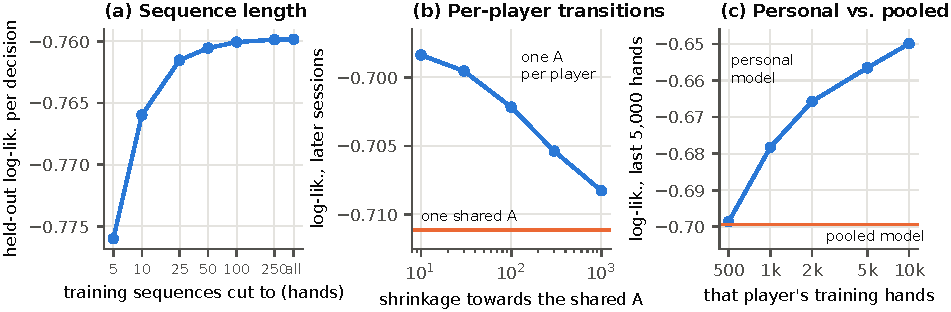
\includegraphics[width=\linewidth]{../figures/fig_ablation.pdf}
\caption{(a) Held-out log-likelihood when training sessions are cut into pieces of a given length. (b) Shared emissions with one transition matrix per player, for different amounts of shrinkage. (c) A personal four-state HMM trained on a player's first $n$ hands against the pooled model, on that player's last 5{,}000 hands (31 high-volume players).}
\label{fig:ablation}
\end{figure}

\begin{table}[h]
\caption{Alphabet and context, $K=4$. All models are scored on the same task: one-step-ahead log-probability of fold / check-call / raise on new players. $V$ is Cram\'er's $V$ between decoded state and position (0 = unrelated).}
\label{tab:abl}
\centering\small
\begin{tabular}{lrrrr}
\toprule
 & Parameters & $K=1$ & $K=4$ & $V$\\
\midrule
3 symbols, no context & 23 & $-0.754$ & $-0.728$ & 0.003\\
8 symbols, no context & 43 & $-0.754$ & $-0.733$ & 0.009\\
3 symbols, with context & 95 & $-0.649$ & $\mathbf{-0.609}$ & 0.005\\
8 symbols, with context (main) & 295 & $-0.649$ & $-0.615$ & 0.009\\
\bottomrule
\end{tabular}
\end{table}

\begin{table}[h]
\caption{Event study on held-out sessions: change in VPIP after a big loss minus change after a big win, in percentage points, with 95\% intervals from a bootstrap over players.}
\label{tab:sub}
\centering\small
\begin{tabular}{lrr}
\toprule
Subset & Big losses & Loss minus win\\
\midrule
All held-out events & 13{,}957 & $+1.04$ $[0.78,1.31]$\\
Stake \$0.25 & 4{,}187 & $+1.41$ $[1.00,1.84]$\\
Stakes \$4 to \$10 & 9{,}770 & $+0.88$ $[0.57,1.19]$\\
Sessions on 1--2 tables & 820 & $+1.49$ $[0.33,2.63]$\\
Sessions on 3 or more tables & 13{,}137 & $+1.01$ $[0.76,1.29]$\\
Players with fewer than 3{,}000 hands & 1{,}702 & $+1.40$ $[0.62,2.20]$\\
Players with 3{,}000 hands or more & 12{,}255 & $+0.99$ $[0.74,1.26]$\\
Threshold 30\,bb & 21{,}233 & $+0.95$ $[0.71,1.18]$\\
Threshold 100\,bb & 7{,}922 & $+1.09$ $[0.76,1.43]$\\
\bottomrule
\end{tabular}
\end{table}

\begin{table}[h]
\caption{Pooled input-output HMM: probability of \emph{staying} in the current state at the next hand, by input, with 95\% bootstrap intervals (200 resamples of training players) for the after-loss row.}
\label{tab:io}
\centering\small
\begin{tabular}{lrrrr}
\toprule
 & S1 & S2 & S3 & S4\\
\midrule
No event & 0.9991 & 0.9985 & 0.9987 & 0.9974\\
After a big win & 0.9977 & 0.9943 & 0.9980 & 0.9939\\
After a big loss & 0.9955 & 0.9944 & 0.9859 & 0.9905\\
\quad 95\% interval & [0.989, 0.999] & [0.980, 0.998] & [0.971, 0.994] & [0.978, 0.997]\\
\bottomrule
\end{tabular}
\end{table}

\begin{table}[h]
\caption{Models with per-player parameters: test log-likelihood per decision (each player's last 30\% of hands; 2.74M decisions).}
\label{tab:personal}
\centering\small\setlength{\tabcolsep}{3.5pt}
\begin{tabular}{lrr}
\toprule
Model & 8 symbols & 3 symbols\\
\midrule
Pooled, no hidden state & $-0.8439$ & $-0.6359$\\
Pooled HMM, $K=4$ / $K=8$ & $-0.7511$ / $-0.7359$ & \\
Per-player table, no hidden state & $-0.6986$ & $-0.5851$\\
\quad + second mode, weak prior ($\kappa_2=20$): no switching / HMM & $-0.7021$ / $-0.7014$ & $-0.5862$ / $-0.5861$\\
\quad + second mode, strong prior ($\kappa_2=320$): no switching / HMM & $-0.6974$ / $-0.6972$ & $-0.5849$ / $-0.5852$\\
\shiftrows
\bottomrule
\end{tabular}
\end{table}

\begin{table}[h]
\caption{Negative control. Personal HMMs with contexts, five-fold cross-validation over sessions; change in log-likelihood per decision relative to $K=1$.}
\label{tab:pluribus}
\centering\small
\begin{tabular}{lrrrrr}
\toprule
Player & Hands & $K=1$ & $K=2$ & $K=3$ & $K=4$\\
\midrule
Pluribus (bot) & 10{,}000 & $-0.6953$ & $-0.0001$ & $-0.0002$ & $-0.0004$\\
MrBlue & 9{,}121 & $-0.7041$ & $-0.0001$ & $-0.0003$ & $-0.0004$\\
MrOrange & 7{,}512 & $-0.6161$ & $-0.0007$ & $-0.0005$ & $-0.0006$\\
Bill & 6{,}713 & $-0.6537$ & $+0.0060$ & $+0.0010$ & $-0.0006$\\
MrPink & 6{,}055 & $-0.6401$ & $-0.0002$ & $-0.0004$ & $-0.0006$\\
Eddie & 5{,}510 & $-0.6864$ & $-0.0011$ & $-0.0013$ & $-0.0007$\\
MrWhite & 4{,}483 & $-0.6555$ & $-0.0003$ & $-0.0005$ & $-0.0008$\\
\midrule
40 PartyPoker players & 10{,}000 each & \multicolumn{4}{l}{best $K>1$: median $-0.0001$; better than $K=1$ for 28\%}\\
\bottomrule
\end{tabular}
\end{table}
